\documentclass{article}
\usepackage[utf8]{inputenc}
\usepackage[french]{babel}

\title{ \bf Compte rendu méthode de conception:  Mystic Robot}
\author{ Aubry Nicolas, Leblond Valentin, Mori Baptiste, Chagneux Dimitri}
\date{ \bf Octobre - Novembre 2018}

\usepackage{natbib}
\usepackage{graphicx}

\begin{document}
\maketitle
\tableofcontents

\vspace{5\baselineskip}

\section{Introduction}
Voici notre jeu, pour la méthode de conception.

\section{Le jeu }

\subsection{Les règles du jeu : }

A chaque tour de jeu, les joueurs jouent l'un après l'autre selon un ordre initialement défini, ou selon
un ordre tiré aléatoirement à chaque tour.

\vspace{1\baselineskip}

\subsubsection{Une action possible est:}

\vspace{1\baselineskip}

\begin{itemize}
    \item  Déplacement d'une case (4 directions possibles seulement).
    \item  Dépôt d'une mine ou d'une bombe sur l'une des 8 cases voisines.
    \item  Utilisation d'un tir horizontal ou d'un tir vertical.
    \item  Déclenchement du bouclier, qui protège des tirs et bombes lors du prochain tour.
    \item  Ne rien faire pour économiser son énergie.
\end{itemize}

\vspace{1\baselineskip}

\subsubsection{La grille :}

La grille peut contenir, lors de sa création, des murs (cases non-utilisables par les combattants et infranchissables par les tirs), et des pastilles d'énergie que les combattants peuvent récupérer en se plaçant dessus.

\vspace{1\baselineskip}

\subsubsection{Les bombes, mines, tirs et shield :}

\vspace{1\baselineskip}

\begin{itemize}
    \item Une mine explose lorsqu'un combattant se place sur la case qu'elle occupe.
    \item Une bombe explose au bout d'un certain délai t (compte à rebours en nombre de tours de jeu),
	et impacte les combattants se trouvant sur l'une des 8 cases voisines, ou , comme une mine,	si l'on se place dessus.
	\item Les bombes et les mines peuvent avoir deux types de visibilité: visible de tous les combattants, ou visible seulement du combattant qui l'a déposée.
	\item Un tir horizontal impacte les combattants se trouvant sur la même ligne horizontale, à un nombre de cases inférieur à la distance d (portée limitée). Idem pour un tir vertical (i.e sur la même
	colonne).
	\item Une explosion ou un tir impactant un combattant fait baisser son énergie d'une certaine valeur qui fera partie des paramètres du jeu.
	\item Un déplacement et l'utilisation du bouclier ont eux aussi leurs coûts respectifs.
    \item Un combattant perd le jeu lorsque son énergie est négative ou nulle. Il disparaît alors du jeu.
    \item Le gagnant est le dernier survivant.
\end{itemize}

\vspace{1\baselineskip}

\section{Diagramme UML du jeu :}

\subsection{Le diagramme :}

\vspace{3\baselineskip}


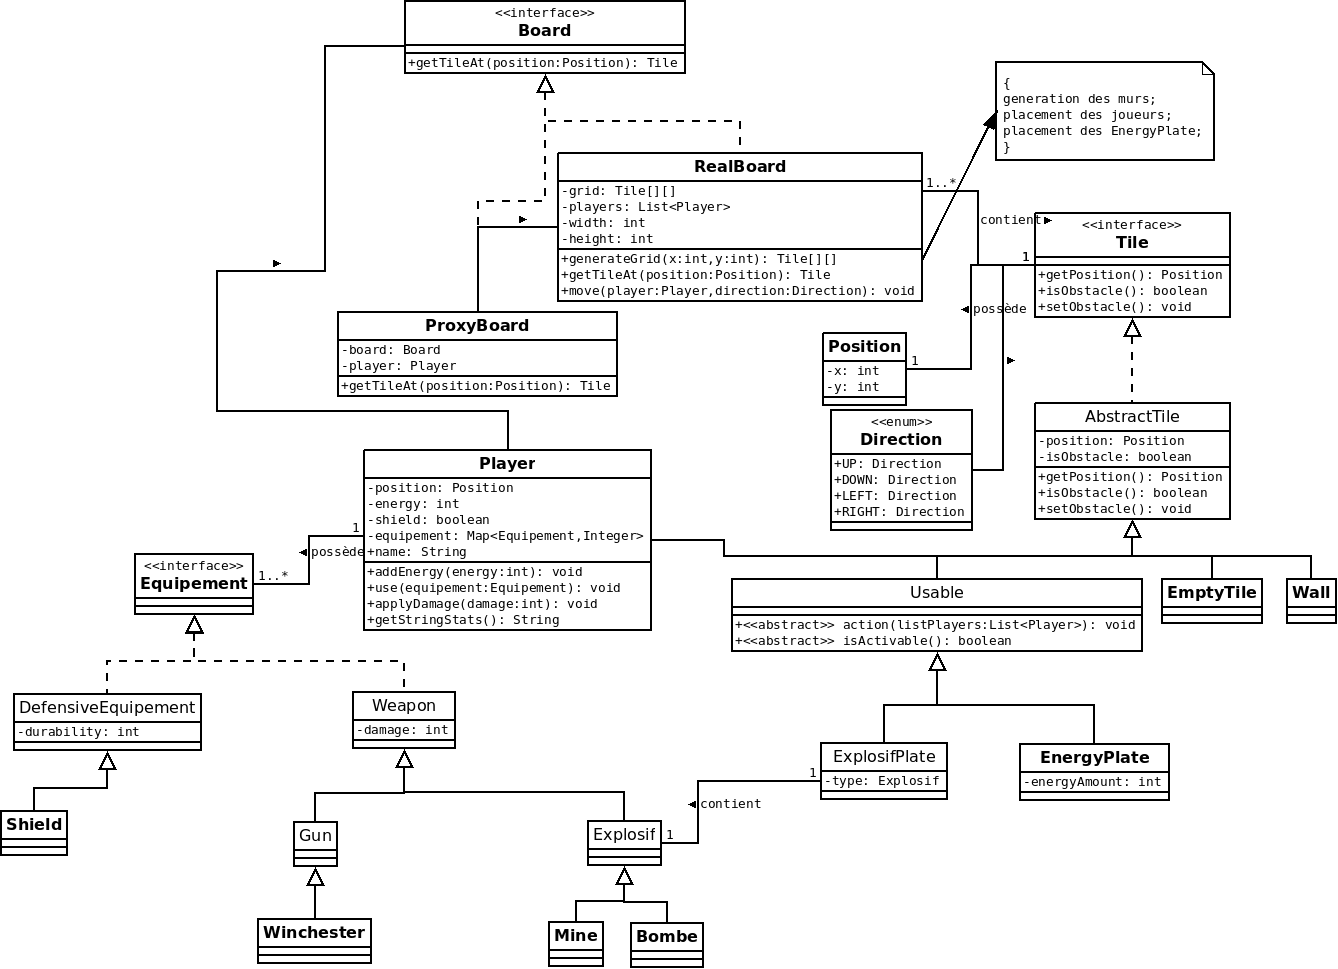
\includegraphics[scale=0.25]{DiagrammeUML.png}


\vspace{1\baselineskip}

\subsection{Explications :}

\vspace{1\baselineskip}

\section{Les patterns et modèles utilisés:}

\subsection{Le pattern Strategy:}


Le pattern Strategy est un pattern qui permet d'externaliser le contenu de certaines méthodes pour pouvoir modifier les comportements soit dynamiquement, soit en utilisant de nouvelles implémentations.


\subsection{Le pattern Factory:}

Le pattern Factory permet de générer dynamiquement des types d'objets.

\vspace{0.3\baselineskip}

Dans notre projet, on se sert du pattern afin de créer des objets Player qui ont des caractéristiques prédéfinies (énergie, stuff, rôle, etc...).
On l'utilise dans la classe RobotFactory, c'est grâce à cela que l'on arrive à dire si on a des joueurs de types sniper, tank ou autres.



\subsection{Le pattern Proxy:}

Le pattern Proxy permet de servir d'intermédiaire entre l'objet à contrôler et celui qui veut y accéder.

\vspace{1\baselineskip}

Dans notre jeu, nous avons implémenté le pattern Proxy, afin de permettre aux différents joueurs de ne pas voir les mines disposées par les ennemis. Mais de voir seulement les mines ou bombes que le joueur a lui-même poser.

\vspace{1\baselineskip}

Voici un exemple de ce que cela peut donner graphiquement :

\begin{figure}[h]
   \caption{\label Exemple d'utilisation du pattern Proxy :}
   \vspace{0.5\baselineskip}
   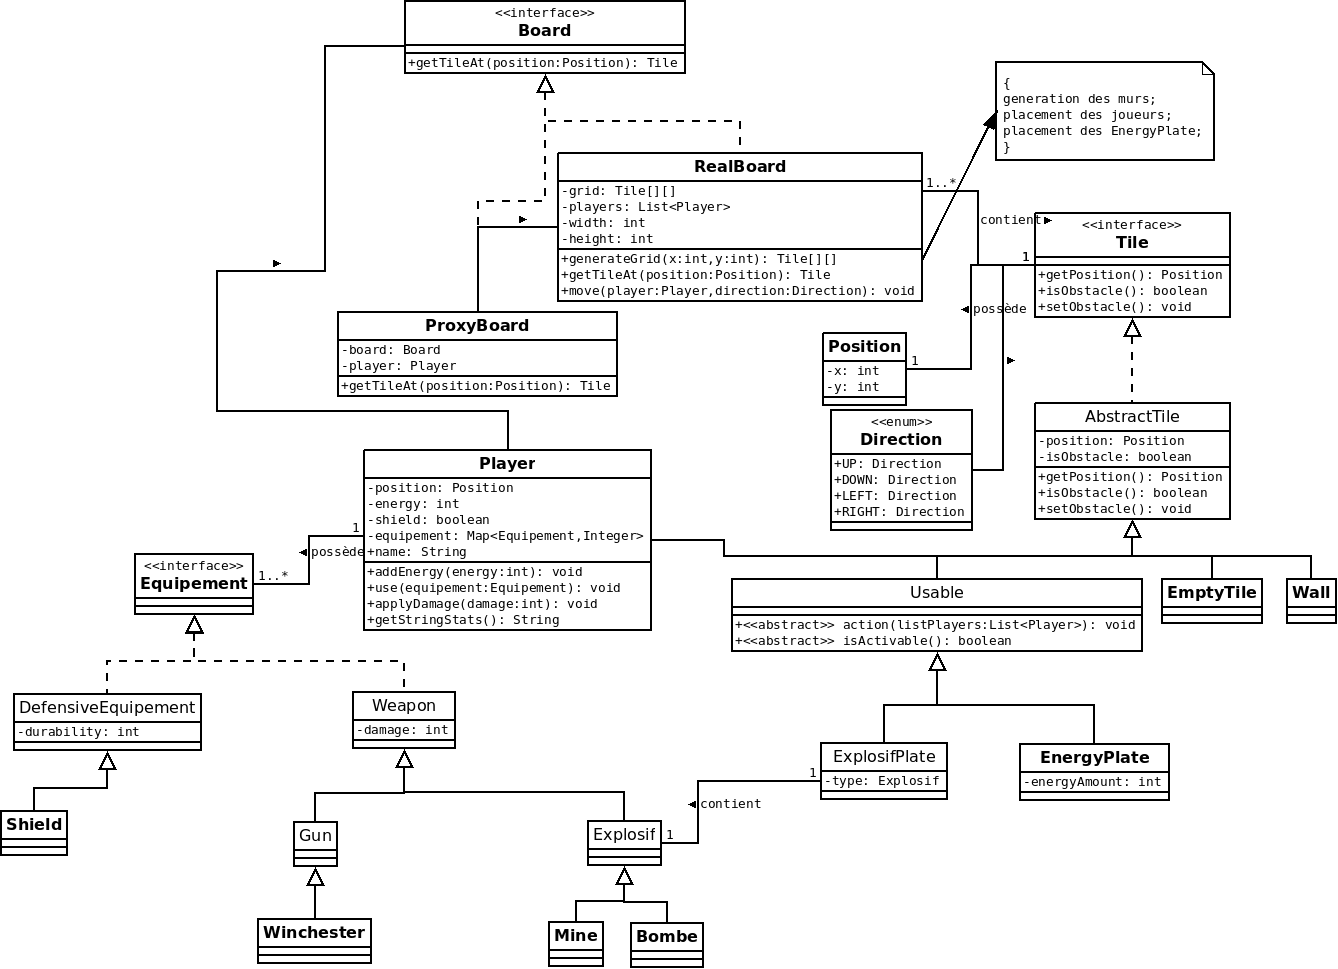
\includegraphics[scale=0.25]{DiagrammeUML.png}
\end{figure}


\subsection{Le pattern Decorator:}

Le pattern Décorator permet d'éviter la redondance et l'explosion du nombre de classes. Donc on créer un objet B qui se fait passer pour un objet A en enrichissant ses fonctionnalités.

\subsection{Le pattern Singleton:}

Le pattern Singleton est un pattern de construction, il permet d'obtenir une instance unique d'une classe.

\subsection{Le modèle MVC:}

Voici notre modèle:

\vspace{1\baselineskip}

Le Modèle : Le modèle de notre application est notre interface graphique.

La Vue : La vue elle nous sert à afficher graphiquement notre jeu.

Le contrôleur :


\section{Test du jeu :}

\section{Conclusion}




\bibliographystyle{plain}
\bibliography{references}

\vspace{1\baselineskip}

Référence aux différents CM et TP de Yann Mathet.
\end{document}
